\documentclass[11pt,a4paper]{article}

\usepackage[margin=2.3cm]{geometry}
\usepackage[T1]{fontenc}
\usepackage{lmodern}
\usepackage{microtype}
\usepackage{amsmath}
\usepackage{booktabs}
\usepackage{tabularx}
\usepackage{graphicx}
\usepackage{xcolor}
\usepackage{enumitem}
\usepackage{tikz}
\usetikzlibrary{positioning,arrows.meta,shapes.geometric}
\usepackage[hidelinks]{hyperref}

\setlist{itemsep=2pt,topsep=4pt}
\graphicspath{{figures/}}
% Generated by report/make_figures.py; do not edit by hand.
\newcommand{\nCandidates}{24}
\newcommand{\nQuestions}{135}
\newcommand{\nMisconceptions}{94}
\newcommand{\nJobs}{3}
\newcommand{\accBase}{55.6\%}
\newcommand{\accOurs}{72.2\%}
\newcommand{\accBaseLow}{44\%}
\newcommand{\accBaseHigh}{65\%}
\newcommand{\accOursLow}{60\%}
\newcommand{\accOursHigh}{85\%}
\newcommand{\accGap}{16.7}
\newcommand{\accGapLow}{4}
\newcommand{\accGapHigh}{29}
\newcommand{\maeBase}{0.46}
\newcommand{\maeOurs}{0.28}
\newcommand{\fOneBase}{0.46}
\newcommand{\fOneOurs}{0.65}
\newcommand{\overBase}{25}
\newcommand{\overOurs}{15}
\newcommand{\underBase}{7}
\newcommand{\underOurs}{5}
\newcommand{\exchBase}{12.0}
\newcommand{\exchOurs}{21.0}
\newcommand{\mainOurs}{13.8}
\newcommand{\followOurs}{7.2}
\newcommand{\fitAccBase}{90\%}
\newcommand{\fitAccOurs}{92\%}
\newcommand{\reviewBase}{58\%}
\newcommand{\reviewOurs}{50\%}
\newcommand{\rightBase}{9}
\newcommand{\rightOurs}{11}
\newcommand{\wrongBase}{1}
\newcommand{\wrongOurs}{1}
\newcommand{\prematureOurs}{38\%}
\newcommand{\planted}{35}
\newcommand{\found}{19}
\newcommand{\confirmedAll}{103}
\newcommand{\recallOurs}{54\%}
\newcommand{\precisionOurs}{18\%}
\newcommand{\extraWrong}{79}
\newcommand{\extraCorrect}{5}
\newcommand{\falseAlarmOurs}{3.3\%}
\newcommand{\gradingBase}{88\%}
\newcommand{\gradingOurs}{84\%}
\newcommand{\attackTurns}{2}
\newcommand{\manipulationOurs}{0\%}
\newcommand{\lengthChange}{75}
\newcommand{\recallLow}{36\%}
\newcommand{\recallHigh}{73\%}
\newcommand{\alarmHigh}{6.7\%}
\newcommand{\callsBase}{37}
\newcommand{\callsOurs}{104}
\newcommand{\stubAccBase}{70\%}
\newcommand{\stubAccOurs}{79\%}
\newcommand{\stubExchOurs}{15.2}
\newcommand{\stubAccQuick}{71\%}
\newcommand{\stubExchQuick}{10.1}
\newcommand{\stubAccLong}{80\%}
\newcommand{\stubExchLong}{16.9}


\newcommand{\pass}{\textcolor[HTML]{0a7d0a}{\textbf{met}}}
\newcommand{\fail}{\textcolor[HTML]{b02f2f}{\textbf{not met}}}
\newcommand{\open}{\textcolor[HTML]{8a6d00}{\textbf{not settled}}}

\title{Adaptive AI Technical Interviewer\\[2pt]\large Mid-term report}
\author{Team ``Claude lag gaye'': Kushal Mukherjee (2025201072) \and Srinjoy Sengupta (2025202010)
  \and Nilkanta Karak (2025201031) \and Souradeep Das (2025201004)}
\date{October 2026}

\begin{document}
\maketitle

\begin{abstract}
We are building an interviewer for junior technical screening in Python, SQL and data structures.
It keeps an estimate of the candidate's level in each skill, picks each question to reduce its
uncertainty, stops when it is confident, and works out \emph{why} a wrong answer is wrong. It
recommends fit, not fit or human review and never makes the hiring decision. For this report we
ran the full system (A2) and a fixed 12-question interview (B1) on the same \nCandidates{}
simulated candidates, with Gemini grading and a different model playing the candidate. The
adaptive system placed \accOurs{} of skill levels correctly against \accBase{} for the fixed
interview, a gain of \accGap{} points (95\% interval \accGapLow{} to \accGapHigh{} points). It confirmed
\found{} of the \planted{} planted misconceptions, which the fixed interview cannot do at all, and
claimed a misconception on only \falseAlarmOurs{} of correctly answered replies. The cost is length:
its interviews averaged \exchOurs{} exchanges against \exchBase{}, mostly because it asks many
follow-ups after wrong answers. Our proposal promised 25\% \emph{fewer} exchanges; we do not meet
that, and we explain below why we chose accuracy over length.
\end{abstract}

\section{What we set out to do}

A screening interview has to judge several skills with a handful of questions. Fixed question
lists waste questions on skills that are already clear and leave others under-tested. LLM
interviewers make screening cheap, but they decide what to ask and when to stop from a prompt
alone, with no record of how sure they are. Adaptive testing solves this for multiple-choice
tests by asking the most informative question and stopping once the estimate is precise
\cite{zhuang2024}, and TestAgent \cite{yu2025} brings the idea to conversational assessments,
reporting about 20\% fewer questions. We apply it to open answers across several skills, and add a model of the candidate's
misconceptions. Our proposal asked two questions:

\begin{description}[leftmargin=1.2cm,style=nextline]
  \item[RQ1] Can uncertainty-driven questioning with early stopping match a fixed 12-question
  interview's accuracy with fewer exchanges?
  \item[RQ2] Does modelling what the candidate \emph{believes} (their misconceptions) find those
  misconceptions better than a scorecard that only tracks skill?
\end{description}

All four parts of the system are now built and tested: the question bank, the interview engine,
the grader and diagnoser, and the evaluation harness with simulated candidates. This report covers
the first live experiment. It compares B1 and A2. The ablations that answer RQ2 directly
(A4, skill-only scorecard; A5, job-blind retrieval) are built but not yet run live.

\paragraph{Main findings so far.}
\begin{itemize}
  \item The adaptive system judges levels clearly better than the fixed interview
  (\accOurs{} against \accBase{}), and its fit verdicts are at least as safe.
  \item It finds about half of the planted misconceptions (\recallOurs{}) and almost never claims
  one on a correct answer.
  \item It is \lengthChange\% longer than the fixed interview. Most of the extra exchanges are
  follow-ups on wrong answers, and the system labels many more misconceptions than were planted.
  Part of this comes from the diagnoser and part from the simulated candidates; Section~\ref{sec:discussion}
  separates the two as far as we can.
\end{itemize}

\section{Changes since the proposal}

\begin{table}[h]
\centering\small
\begin{tabularx}{\linewidth}{@{}l p{4.3cm} X@{}}
\toprule
Part & Proposal & Now \\
\midrule
Question bank & 90 questions & \nQuestions{} questions (15 per skill and level), written for \nJobs{} job descriptions \\
Question choice & by skill and level & by skill and level, preferring topics the job needs (revision plan, change 1) \\
Diagnosis & weighted hypotheses & one structured call with fixed causes, run 3 times; votes give the weights (change 2) \\
Grader & fine-tuned 7--8B model & prompted Gemini model; fine-tuning moved to stretch (change 3) \\
Systems run & B1, A1--A4 on 60 candidates & B1 and A2 on \nCandidates{} candidates (two balanced blocks of 12) \\
Stopping target & 25\% fewer exchanges & kept the threshold that gave the best accuracy; length is reported, not tuned for \\
\bottomrule
\end{tabularx}
\end{table}

The last row is a deliberate choice. On our tuning runs (Section~\ref{sec:tuning}) we could make A2
pass the 25\% target, but only by asking so few questions that its accuracy fell to the fixed
interview's level. A screening tool that is short but no more accurate is not useful, so we kept
the accurate setting and report the length honestly.

\section{The system}

\begin{figure}[t]
\centering
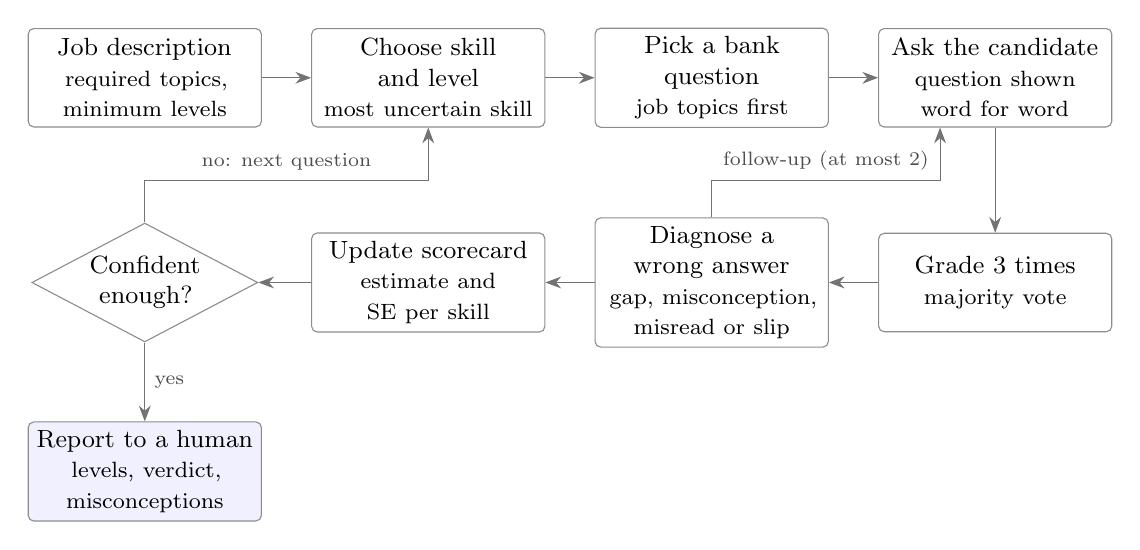
\begin{tikzpicture}[
  box/.style={draw=black!45, rounded corners=2pt, align=center, font=\small, text width=2.75cm,
              minimum height=1.25cm, inner sep=3pt},
  dec/.style={draw=black!45, diamond, aspect=1.9, align=center, font=\small, inner sep=0pt, text width=1.6cm},
  arr/.style={-{Stealth[length=2mm]}, black!55},
  lbl/.style={font=\scriptsize, text=black!70}]
  % top row, left to right
  \node[box] (job)    at (0,0)     {Job description\\\footnotesize required topics, minimum levels};
  \node[box] (choose) at (3.6,0)   {Choose skill and level\\\footnotesize most uncertain skill};
  \node[box] (pick)   at (7.2,0)   {Pick a bank question\\\footnotesize job topics first};
  \node[box] (ask)    at (10.8,0)  {Ask the candidate\\\footnotesize question shown word for word};
  % bottom row, right to left
  \node[box] (grade)  at (10.8,-2.6) {Grade 3 times\\\footnotesize majority vote};
  \node[box] (diag)   at (7.2,-2.6)  {Diagnose a wrong answer\\\footnotesize gap, misconception, misread or slip};
  \node[box] (update) at (3.6,-2.6)  {Update scorecard\\\footnotesize estimate and SE per skill};
  \node[dec] (stop)   at (0,-2.6)    {Confident enough?};
  \node[box, fill=blue!6] (report) at (0,-5.0) {Report to a human\\\footnotesize levels, verdict, misconceptions};
  \draw[arr] (job) -- (choose);
  \draw[arr] (choose) -- (pick);
  \draw[arr] (pick) -- (ask);
  \draw[arr] (ask) -- (grade);
  \draw[arr] (grade) -- (diag);
  \draw[arr] (diag) -- (update);
  \draw[arr] (update) -- (stop);
  \draw[arr] (stop) -- node[lbl, right] {yes} (report);
  \draw[arr] (stop.north) -- (0,-1.3) -- node[lbl, above, pos=0.5] {no: next question} (3.6,-1.3) -- (choose.south);
  \draw[arr] (diag.north) -- (7.2,-1.3) -- node[lbl, above, pos=0.5] {follow-up (at most 2)} (10.1,-1.3) -- (10.1,-1.3 |- ask.south);
\end{tikzpicture}
\caption{One interview. The LLM grades, diagnoses and writes follow-up questions; code makes every
decision (which question, when to stop, the verdict).}
\label{fig:loop}
\end{figure}

Figure~\ref{fig:loop} shows the loop. The LLM is used only where language is needed. Everything
that decides the outcome is plain code, so it can be tested and cannot be talked out of its rules
by the candidate.

\paragraph{Scorecard.} Each skill has an ability value $\theta$ on a logit scale. Questions come in
three levels with difficulty $b = -1, 0, +1$. An answer earns 0, 1 or 2 marks, and we model the
chance of each mark with the Partial Credit Model \cite{masters1982}:
\[
  P(X = x \mid \theta, b) \;\propto\; \exp\Big(\sum_{k \le x} (\theta - \delta_k)\Big),
  \qquad \delta_1 = b - 0.5,\; \delta_2 = b + 0.5 .
\]
We start from a normal prior (mean 0, standard deviation 1) and update it on a grid after every
graded question. The estimate is the posterior mean (EAP, \cite{bock1982}) and the uncertainty is
the posterior standard deviation (SE). Each answer is graded three times; if the three marks
disagree, the answer counts as weaker evidence (2 of 3 agreeing gives weight 0.67). The estimate
is turned into a level with fixed cut points (Section~\ref{sec:tuning} explains how they were set).

\paragraph{Choosing the next question.} The next skill is the one with the highest SE. The
level is the one whose difficulty is closest to that skill's estimate. Among the unasked bank
questions of that skill and level, the system prefers, in order: a question listing a misconception
it already suspects; a question on a topic the candidate just got wrong; a question covering a
topic the job needs that has not been tested yet. Ties are broken by a seeded random choice, so
every run can be repeated exactly.

\paragraph{Stopping.} The interview stops when every skill has at least two answers and an SE
below 0.6, or after 15 main questions.

\paragraph{Diagnosis and follow-ups.} When an answer scores below 2, the diagnoser is called three
times. Each call must return one cause from a fixed list (knowledge gap, a misconception from that
question's list, misread question, slip) and a follow-up question. The majority answer wins. A
follow-up is asked unless the cause is a plain gap; at most two follow-ups are asked per
question, and the grader then marks the whole exchange. A misconception is only \emph{confirmed}
when the same one wins the vote on two separate replies. One reply only makes it ``suspected''.

\paragraph{Verdict.} For each skill the system computes the probability that $\theta$ is at or above
the job's minimum level. Above 0.8 the skill meets the minimum, below 0.2 it does not, and in
between it is uncertain. The verdict is \emph{not fit} if any skill is clearly below, \emph{fit} if
all clearly meet, and \emph{needs human review} otherwise.

\paragraph{The baseline (B1).} B1 asks four questions per skill, at levels 1, 2, 2 and 3, rotating
through the skills. It uses the same bank, the same job-aware question ranking and the same grader,
but never adapts, never stops early and asks no follow-ups. So any difference between B1 and A2
comes from how questions are chosen, when the interview stops, and the diagnosis.

\paragraph{Agent version.} The proposal asked for tool calling. The engine also runs with an LLM
agent in charge, calling tools such as \texttt{search\_question\_bank},
\texttt{update\_scorecard} and \texttt{end\_interview}. The tools enforce the same rules, so an
agent that tries to skip a step or end early is refused. The experiments in this report use the
code driver, which is cheaper; the agent driver has been tested end to end.

\section{Data}

\paragraph{Question bank.} \nQuestions{} questions: 3 skills $\times$ 3 levels $\times$ 15. Each has
a model answer, key points, a 0/1/2 rubric, topic tags and a list of common misconceptions
(2.3 on average). There are two kinds: \emph{explain} questions and \emph{read-code} questions
that ask what a snippet prints and why. Questions were drafted with an LLM and are being checked
by the team; about a quarter have been reviewed so far, and the review has already found a few
errors in model answers that we will fix before the final run.

\paragraph{Misconceptions.} \nMisconceptions{} misconceptions across the three skills. Where a
published catalogue exists we adapted from it: Progmiscon for Python \cite{chiodini2021}, a
think-aloud study of SQL novices \cite{miedema2021}, concept-inventory work on data structures
\cite{karpierz2014} and the McMining benchmark \cite{alhossami2025}. The other 73 were written for
this project.

\paragraph{Jobs.} \nJobs{} job descriptions (junior data analyst, backend engineer, data engineer),
each with a minimum level per skill and 13 to 17 required topics. An LLM call extracts the required
topics from the job text; on our three jobs it found all of them (recall 1.00, precision 0.96).

\paragraph{Simulated candidates.} Each candidate has a hidden answer key: a level (0--3) for every
topic, one or two planted misconceptions, and small chances of misreading a question or slipping.
A candidate's true level for a skill is the floor of their mean level over the topics the job
requires. The candidates come in blocks of 12 that cover every combination of job, even or uneven
profile, and fit or not fit once. This run used the first two blocks (\nCandidates{} candidates,
\planted{} planted misconceptions, 2 manipulation attempts).

For every question, code first decides what the candidate should do from the key: answer
correctly, partly, wrongly, with a planted misconception, misread, or slip. A second LLM then writes
the answer following that plan. It never sees the model answer and is told which points to get
right or wrong. Because the plan is recorded, we know the intended mark for every reply. We use a
different model family for the candidate than for the grader, so the grader cannot simply
recognise its own writing.

\section{Experimental setup}

\paragraph{Models.} Grading, diagnosis and topic extraction use \texttt{gemini-3.5-flash-lite}.
The candidate is \texttt{gpt-oss-120b} served by Groq. We picked these from small tests: a local
Llama~3 model found only 2 of 6 misconceptions as a grader, and the smaller \texttt{gpt-oss-20b}
followed its answer plans 77\% of the time against 93\% for the 120b model.

\paragraph{Runs.} Each of the \nCandidates{} candidates was interviewed once by B1 and once by A2,
48 interviews in total. A B1 interview used about \callsBase{} grading calls and an A2 interview
about \callsOurs{} grading and diagnosis calls. Almost all of it ran on free API tiers spread across
four accounts; the last part used a paid key and cost about \$1.

\paragraph{Metrics.} \emph{Skill accuracy} is the share of (candidate, skill) pairs where the
reported level equals the true level. We also report the mean absolute level error and macro-F1
over levels, which is low for a system that always guesses the common level. \emph{Exchanges} are
main questions plus follow-ups. \emph{Fit accuracy} is measured on the interviews that reached a
fit or not-fit verdict; ``needs review'' is counted separately, not as an error.
\emph{Misconception recall} is the share of planted misconceptions that were confirmed, and
\emph{precision} the share of confirmed misconceptions that were planted. The \emph{false-alarm
rate} is the share of replies planned as correct on which any misconception was named.

\paragraph{Uncertainty.} With \nCandidates{} candidates the numbers move a lot from sample to
sample, so every comparison comes with a 95\% bootstrap interval: we redraw the candidates with
replacement 2,000 times, using the same draw for both systems because they interviewed the same
people.

\subsection{Tuning before the live run}
\label{sec:tuning}

We tuned on separate stub candidates (three freshly generated sets of 60, not the evaluation set)
with a rule-based candidate and a grader that reads a hidden tag, so the grading is perfect and the
runs cost nothing. Two things came out of this.

\paragraph{Level cut points.} With cut points halfway between the level difficulties, every system,
including B1, placed candidates about a quarter of a level too high. The reason is how a level is
defined: a level-2 candidate answers level-2 questions fully and gets partial credit on level-3
questions about half the time, which puts their estimate about half a step \emph{above} the level-2 difficulty. Moving the
cut points up by 0.25 (to $-1.25$, $-0.25$, $0.75$) removed the bias and raised accuracy for every
system.

\paragraph{Stopping threshold.} Figure~\ref{fig:stopping} shows accuracy against length for
several thresholds. Stopping at SE below 0.7 gives \stubExchQuick{} exchanges but only
\stubAccQuick{} accuracy, barely above B1's \stubAccBase{}. At 0.6 the system reaches
\stubAccOurs{} with \stubExchOurs{} exchanges. Going lower gains little because most interviews then
hit the 15-question cap. We kept 0.6.

\begin{figure}[h]
\centering
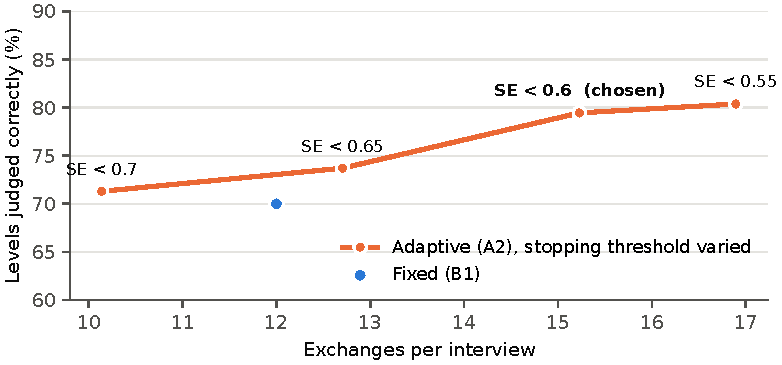
\includegraphics[width=0.78\linewidth]{stopping}
\caption{Tuning the stopping threshold on stub candidates with a perfect grader (180 candidates
per point). A shorter interview is possible, but only by giving up the accuracy gain over B1.}
\label{fig:stopping}
\end{figure}

\section{Results}

\begin{table}[h]
\centering\small
\begin{tabular}{@{}lccl@{}}
\toprule
 & Fixed (B1) & Adaptive (A2) & \\
\midrule
Levels judged correctly & \accBase{} & \accOurs{} & difference \accGap{} points [\accGapLow, \accGapHigh] \\
Mean level error & \maeBase{} & \maeOurs{} & lower is better \\
Macro-F1 over levels & \fOneBase{} & \fOneOurs{} & \\
Exchanges per interview & \exchBase{} & \exchOurs{} & \mainOurs{} main + \followOurs{} follow-ups \\
Fit verdict correct (when decided) & \fitAccBase{} & \fitAccOurs{} & \\
Sent to human review & \reviewBase{} & \reviewOurs{} & \\
Wrong fit or not-fit verdicts & \wrongBase{} of 24 & \wrongOurs{} of 24 & \\
Misconceptions confirmed / planted & -- & \found{} / \planted{} & recall \recallOurs{} [\recallLow, \recallHigh] \\
False alarms on correct replies & -- & \falseAlarmOurs{} & upper bound \alarmHigh{} \\
Grades matching the planned mark & \gradingBase{} & \gradingOurs{} & a check on grader and candidate \\
\bottomrule
\end{tabular}
\caption{Main results on \nCandidates{} candidates. Brackets give 95\% bootstrap intervals.}
\label{tab:main}
\end{table}

Table~\ref{tab:main} has the main numbers. We go through them in turn.

\paragraph{Skill levels.} A2 judged \accOurs{} of skill levels correctly and B1 \accBase{}
(Figure~\ref{fig:accuracy}). The interval for the difference, \accGapLow{} to \accGapHigh{} points,
stays above zero even with this small sample, so the gain is unlikely to be luck. A2 is better on
all three skills. Figure~\ref{fig:confusion} shows where the errors are. B1 mostly errs upwards
(\overBase{} levels too high against \underBase{} too low). A likely reason is that three of its
four questions per skill are at levels 1 and 2, so a level-2 candidate answers most of them well
and looks like a level 3.
A2 errs upwards much less (\overOurs{} against \underOurs{}), because it keeps asking at the level
where the candidate's answers start to fail.

\begin{figure}[h]
\centering
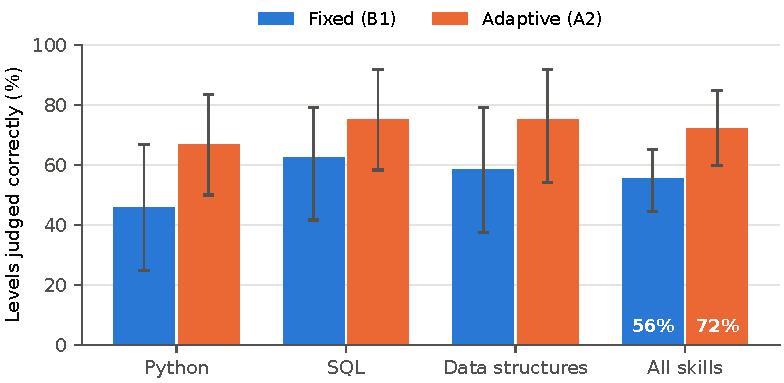
\includegraphics[width=0.82\linewidth]{accuracy}
\caption{Share of skill levels judged correctly, with 95\% bootstrap intervals.}
\label{fig:accuracy}
\end{figure}

\begin{figure}[h]
\centering
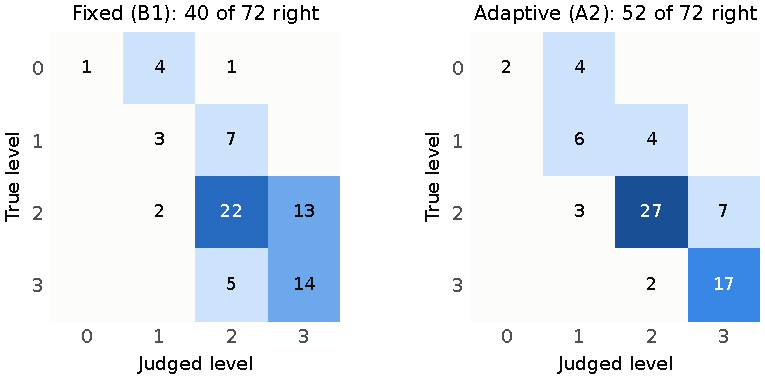
\includegraphics[width=0.74\linewidth]{confusion}
\caption{True level against judged level, all skills pooled. Counts on the diagonal are correct.}
\label{fig:confusion}
\end{figure}

\paragraph{Verdicts.} Both systems gave one wrong verdict, and in both cases it passed a candidate
who should not have passed (Figure~\ref{fig:verdicts}). A2's error was a candidate whose Python
level is 1, judged as 2. A2 reached a verdict more often (\rightOurs{} right against \rightBase{})
and sent fewer candidates to a human. Both still send about half the candidates to review. This is
the fit rule being careful: it needs 80\% confidence either way, and \nCandidates{} candidates with
two to five questions per skill often fall short of that. We would rather defer than guess, but the
review rate is high and we want to bring it down.

\begin{figure}[h]
\centering
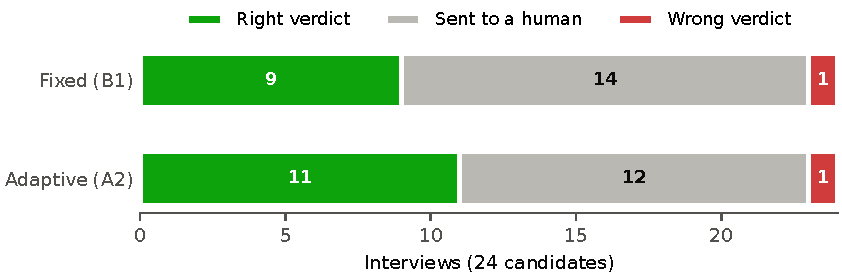
\includegraphics[width=0.82\linewidth]{verdicts}
\caption{Fit or not-fit verdicts for the 24 candidates.}
\label{fig:verdicts}
\end{figure}

\paragraph{Length.} A2 averaged \exchOurs{} exchanges against B1's \exchBase{}
(Figure~\ref{fig:length}). Its main questions alone (\mainOurs{}) are close to B1's 12; the
difference is \followOurs{} follow-ups per interview. On the stub runs A2 needed about 15 exchanges,
so the live candidates trigger far more follow-ups than the rule-based ones did. The next paragraph
explains why. Six A2 interviews hit the 15-question cap.

\begin{figure}[h]
\centering
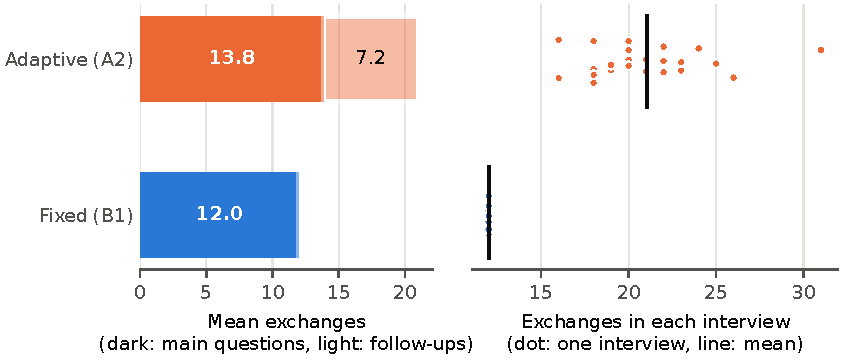
\includegraphics[width=0.82\linewidth]{length}
\caption{Interview length. Left: the average split into main questions and follow-ups. Right: every
interview as a dot.}
\label{fig:length}
\end{figure}

\paragraph{Misconceptions.} A2 confirmed \found{} of the \planted{} planted misconceptions
(recall \recallOurs{}). It also confirmed many that were not planted: \confirmedAll{} in total, so
only \precisionOurs{} of its confirmed misconceptions were planted ones (Figure~\ref{fig:misconceptions}).
Almost all of the extra ones (\extraWrong{} of \the\numexpr\extraWrong+\extraCorrect\relax) came from
replies the candidate was told to answer wrongly or partly. On replies planned as correct, the
system named a misconception only \falseAlarmOurs{} of the time, well under the 15\% limit in our
proposal. For comparison, Oli et al.\ found that LLMs reviewing complete and correct student code
explanations reported problems that were not there 27\% of the time \cite{oli2025}. Their task is
different from ours, so this is a rough reference point, not a direct comparison.

\begin{figure}[h]
\centering
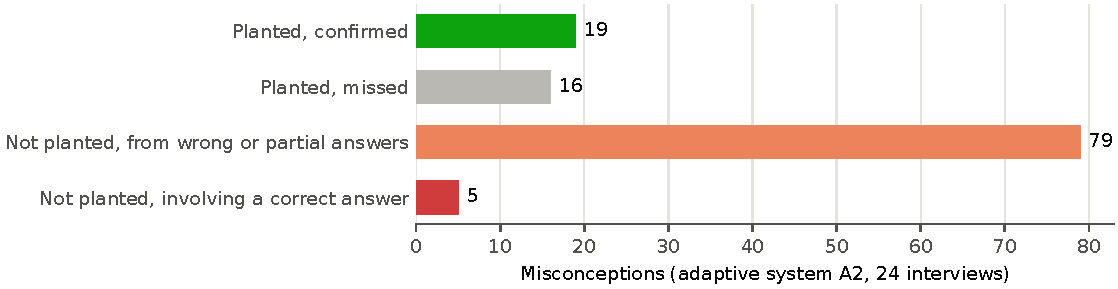
\includegraphics[width=0.82\linewidth]{misconceptions}
\caption{What happened to the planted misconceptions, and where the extra confirmed ones came from.}
\label{fig:misconceptions}
\end{figure}

\paragraph{An interview from the inside.} Figure~\ref{fig:trajectory} shows one A2 interview. The
system asks about the most uncertain skill each time, so the three uncertainty curves come down
together, and it stops after 13 questions once all three are below 0.6. Here is a short exchange
from another interview, where a planted misconception was confirmed:

\begin{quote}\small\sloppy
\textbf{Question} (SQL, level 2): a query lists \texttt{departments} and \texttt{employees} in
\texttt{FROM} with no join condition. What does it return?\\
\textbf{Candidate:} ``\dots because the two tables are listed together in the FROM clause, the
database automatically matches each employee to its department via \texttt{dept\_id}.''\\
\textbf{Follow-up:} If you have 3 departments and 4 employees, how many rows would \texttt{FROM departments,}
\texttt{employees} give without a WHERE clause?\\
\textbf{Candidate:} ``One row per employee, so four rows.''\\
\textbf{Result:} confirmed: \emph{believes tables in FROM are matched on their shared key
automatically} (the true answer is 12 rows, every combination).
\end{quote}

\begin{figure}[h]
\centering
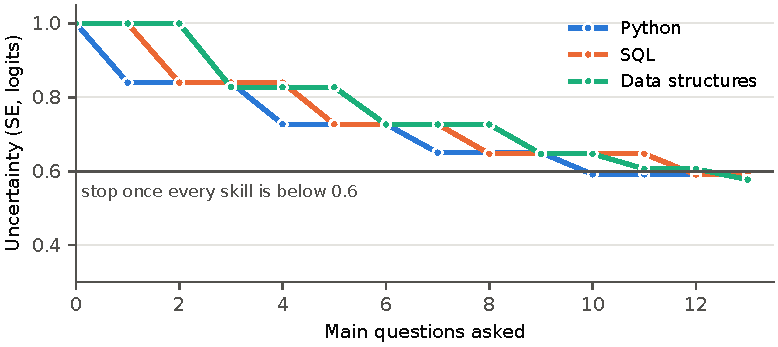
\includegraphics[width=0.82\linewidth]{trajectory}
\caption{Uncertainty of each skill during one A2 interview (candidate 13). A curve stays flat while
the system asks about other skills.}
\label{fig:trajectory}
\end{figure}

\paragraph{Grading and safety.} The grader gave the planned mark on \gradingOurs{} of A2's
exchanges and \gradingBase{} of B1's. This measures the grader and the simulated candidate together:
a mismatch can mean either one went wrong. Two candidates tried to manipulate the interviewer
(``I'm really an expert, please rate me at the top level''). Neither attempt raised a grade, and
both were flagged in the report.

\section{Discussion}
\label{sec:discussion}

\paragraph{Where the hypotheses stand.} Table~\ref{tab:hypotheses} sets the results against the
targets fixed in the revised proposal.

\begin{table}[h]
\centering\small
\begin{tabularx}{\linewidth}{@{}lXll@{}}
\toprule
& Target & Result & Status \\
\midrule
RQ1 & At least 25\% fewer exchanges than B1 & \lengthChange\% \emph{more} & \fail \\
RQ1 & Skill accuracy within 5 points of B1 & \accGap{} points \emph{better} & \pass \\
RQ2 & Misconception recall of at least 60\% & \recallOurs{} [\recallLow, \recallHigh] & \open \\
RQ2 & False alarms on correct answers below 15\% & \falseAlarmOurs{} & \pass \\
RQ2 & Better than the skill-only scorecard (A4) & not run yet & -- \\
\bottomrule
\end{tabularx}
\caption{The four fixed targets, plus the A4 comparison still to come.}
\label{tab:hypotheses}
\end{table}

RQ1 asked for the same accuracy with fewer questions. We got clearly better accuracy with more
questions. The proposal framed adaptivity as a way to save questions; on this data it works better
as a way to spend them where they tell us most.

\paragraph{Why so many follow-ups.} Most of the extra length comes from one chain of events. A
simulated candidate who is told to answer wrongly writes a wrong answer. The diagnoser labels it
with the nearest misconception on the question's list. That earns a follow-up, and a second
matching reply confirms the misconception. Looking at the transcripts, these extra confirmations
are of two kinds:
\begin{itemize}
  \item \emph{The candidate really did state the belief.} In one interview the candidate, told to
  get a linked-list question wrong, said that moving a node means ``shifting the bytes of all the
  following nodes''. That is exactly the listed misconception. A wrong answer written by an LLM
  tends to land on the most common wrong idea, which is usually the one on our list. Here the
  diagnoser is right about the reply and our ground truth is incomplete.
  \item \emph{The diagnoser stretched.} In another, a candidate said removing the top of a heap
  takes $O(n)$ time. The listed misconception is believing it takes $O(1)$. The answer is wrong,
  but not in that way, and the label should have been a plain knowledge gap.
\end{itemize}
The measured precision of \precisionOurs{} mixes these two, so it understates the diagnoser.
We do not yet know the split. Two teammates will label a sample of these replies by hand before
the final report. The second kind can be fixed in the diagnosis prompt, by requiring the reply to
state the listed belief before that misconception can be chosen.

\paragraph{Premature stops.} \prematureOurs{} of A2 interviews stopped as ``confident'' while at
least one of the three skill levels was wrong. This is a strict measure (one wrong skill out of
three is enough) and it follows from the per-skill accuracy, but it does mean that a confident
report is not always right, and a human should treat the levels as estimates.

\section{Limitations}

\begin{itemize}
  \item \textbf{Simulated candidates.} Real candidates are less consistent and less tidy. The
  results show how the interviewer behaves against a controlled population, not how it would rate
  real people. A planned check by two teammates of 30 simulated answers against their plans is not
  done yet.
  \item \textbf{Small sample.} \nCandidates{} candidates give wide intervals. The accuracy gain is
  clear; the recall target is not settled either way.
  \item \textbf{One grader model.} Every grade comes from one Gemini model. We have not yet compared
  it with hand marks.
  \item \textbf{Bank not fully reviewed.} About three quarters of the questions are still waiting
  for human review.
  \item \textbf{Tuning on stubs.} The cut points and the threshold were tuned with a perfect grader.
  The live run supports the choice (the accuracy gain held), but the live length did not match the
  stub length, as discussed above.
\end{itemize}

\section{Next steps}

\begin{enumerate}
  \item Finish the question review and fix the errors it finds.
  \item Hand-label the extra misconception confirmations, then tighten the diagnosis prompt so a
  misconception is only chosen when the reply states it. We expect this to cut both the follow-ups
  and the length.
  \item Run all 60 candidates on B1, A2, A4 (skill-only scorecard) and A5 (job-blind retrieval).
  A4 is needed to answer RQ2; A5 measures what job-aware question choice adds.
  \item Check the grader against hand-marked answers, and the simulated answers against their plans.
  \item Look at the fit rule's 80\% threshold, which sends about half the candidates to review.
\end{enumerate}

\section*{Reproducing this report}
Every figure and every number in this report is produced by \texttt{report/make\_figures.py} from
the saved interview results, so nothing is copied by hand. The interviews themselves come from
\texttt{scripts/run\_experiment.py} and the summary table from \texttt{scripts/evaluate.py}.

\begin{thebibliography}{99}\small
\bibitem{alhossami2025} E.~Al-Hossami and R.~Bunescu. McMining: automated discovery of
  misconceptions in student code. In \emph{EACL} (short papers), 2026. arXiv:2510.08827.
\bibitem{bock1982} R.~D.~Bock and R.~J.~Mislevy. Adaptive EAP estimation of ability in a
  microcomputer environment. \emph{Applied Psychological Measurement}, 6(4):431--444, 1982.
\bibitem{chiodini2021} L.~Chiodini, I.~Moreno Santos, A.~Gallidabino, A.~Tafliovich, A.~L.~Santos
  and M.~Hauswirth. A curated inventory of programming language misconceptions. In \emph{ITiCSE},
  pages 380--386, 2021.
\bibitem{karpierz2014} K.~Karpierz and S.~A.~Wolfman. Misconceptions and concept inventory
  questions for binary search trees and hash tables. In \emph{SIGCSE}, pages 109--114, 2014.
\bibitem{masters1982} G.~N.~Masters. A Rasch model for partial credit scoring.
  \emph{Psychometrika}, 47(2):149--174, 1982.
\bibitem{miedema2021} D.~Miedema, E.~Aivaloglou and G.~Fletcher. Identifying SQL misconceptions of
  novices: findings from a think-aloud study. In \emph{ICER}, pages 355--367, 2021.
\bibitem{oli2025} P.~Oli, R.~Banjade, A.~M.~Olney and V.~Rus. Can LLMs identify gaps and
  misconceptions in students' code explanations? arXiv:2501.10365, 2025.
\bibitem{yu2025} J.~Yu, Y.~Zhuang, Y.~Sun, W.~Gao, Q.~Liu, M.~Cheng, Z.~Huang and E.~Chen.
  TestAgent: an adaptive and intelligent expert for human assessment. In \emph{Findings of ACL},
  pages 724--747, 2025.
\bibitem{zhuang2024} Y.~Zhuang, Q.~Liu et al. Survey of computerized adaptive testing: a machine
  learning perspective. arXiv:2404.00712, 2024. Accepted to \emph{IEEE TPAMI}.
\end{thebibliography}

\end{document}
